\clearpage
\section{Viterbi algorithm, Belief propagation}

\subsection{Hidden Markov Model}
\begin{itemize}
	\item Data: $D = \{x_t\}_{t=1}^T$
	\item Parameters
	\begin{itemize}
		\item Hidden states: $Z = \{z_t\}_{t=1}^T$, where $z_t \in S = \{1,2,\ldots s_\text{max}\}$
		\item Prior probability: $w = \{w_s\}_{s\in S}$, where $w_s \in [0,1]$, such that $\sum_s w_s = 1$.
		\item Transition probabilities: $\{A_{s, r}\}_{s,r\in S}$, where $A_{s,r} \in [0,1]$, such that $\sum_r A_{s,r} = 1$, for all $s$.
		\item Emission probabilities: $\{B_s(x)\}_{s\in S}$, where $B_s(x)$ is a probability density of $x$, i.e. $x\mapsto \mathds{R}$, and $\sum_x B_s(x) = 1$, for all $s$.
	\end{itemize}
	\item Model:
	\begin{itemize}
		\item level 1: $P(x_t\;|\;z_t, B) = B_{z_t}(x_t)$
		\item level 2: $P(Z\;|\;w, A) = P(z_1\;|\; w) \prod_{t=2}^T P(z_t\;|\;z_{t-1}, A) = w_{z_1} \prod_{t=2}^T A_{z_{t-1}, z_{t}}$
	\end{itemize}
	\begin{figure}[h]
	\centering
		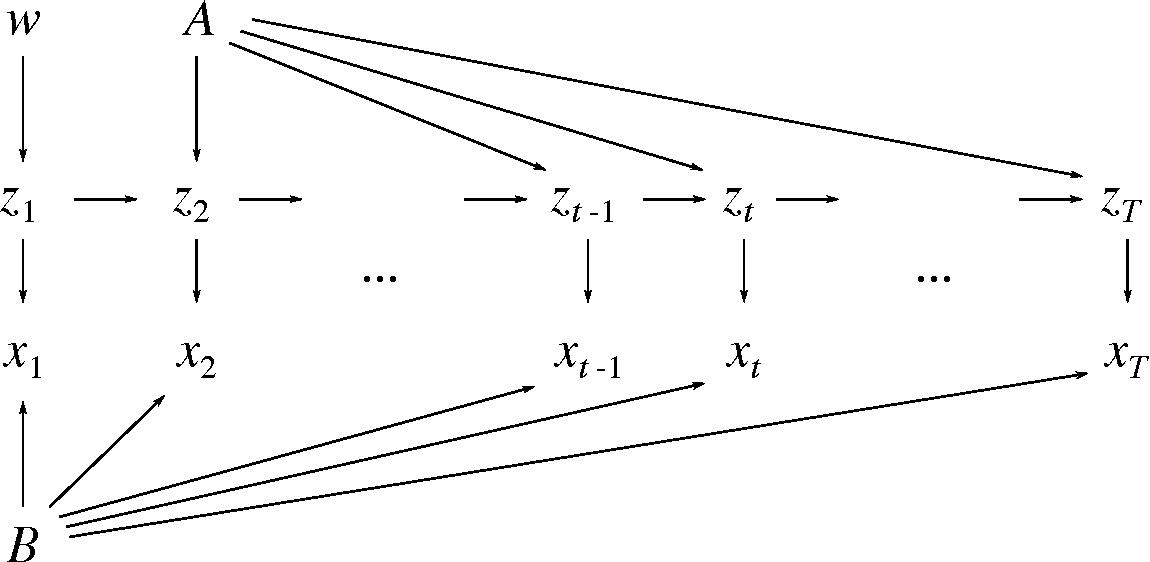
\includegraphics[width=0.5\textwidth]{./figs/09-HMM.pdf}
	\end{figure}

	\item Joint
	\be
		P(D, Z\;|\;w, A, B) = P(D\;|\;Z, B) P(Z\;|\;w, A) = \left[\prod_{t=1}^T B_{z_t}(x_t)\right] \times \left[w_{z_1} \prod_{t=2}^T A_{z_{t-1}, z_{t}}\right]
	\ee
	\item Most likely sequence of states: 
	\be
		Z_\text{MLE} = \amax_Z P(D, Z\;|\;w, A, B) =  \text{(see ``Viterbi algorithm'' below)}
	\ee
	\item Marginal likelihood, marginals of $z_t$ and joint marginal of $(z_{t-1}, z_{t})$:
	\be
		\left.
		\begin{array}{l}
			P(D\;|\;w, A, B) = \sum_Z P(D, Z\;|\;w, A, B) \\
			P(z_t\;|\; D, w, A, B) = \sum_{Z\setminus \{z_t\}} P(D, Z\;|\;w, A, B) \\
			P(z_{t-1}, z_{t}\;|\; D, w, A, B) = \sum_{Z\setminus \{z_{t-1},z_t\}} P(D, Z\;|\;w, A, B)
		\end{array}
		\right\}
		= \text{(see ``Belief propagation'' below)}
	\ee
	\item Maximum-likelihood estimate of level 2 parameters
	\be
		(w, A, B)_\text{MLE} = \amax_{w, A, B} P(D\;|\;w, A, B) = \text{(see ``Baum-Welch'' algorithm below)}
	\ee
\end{itemize}

\newpage
\subsection{Viterbi algorithm}
\no Inputs:
\begin{itemize}
	\item $f_1(s) := P(x_1, z_1=s\;|\;w, B) = w_s B_s(x_1)$, for $s\in S$
	\item $f_t(r, s) := P(x_t, z_t=s\;|\;z_{t-1}=r, A, B) = A_{r,s} B_s(x_t)$, for $t = 2,3,\ldots T$, and $r, s \in S$
	\item $F(Z) := f_1(z_1)\prod_{t=2}^T f_{t}(z_{t-1}, z_t)$
\end{itemize}
Outputs:
\begin{itemize}
	\item $F_\text{max} := \max_Z P(D, Z\;|\;w, A, B) = \max_Z F(Z)$
	\item $(z_1\s, z_2\s, \ldots z_T\s) := Z_\text{MLE} = \amax_Z F(Z)$
\end{itemize}
Algorithm:
\begin{enumerate}
	\item {\bf ``Discover''}\\
	For $s \in S$: 
		\ba
			\phi_1(s) &:=& f_1(s) \hspace{9cm}
		\ea
	For $t \in [2,3,\ldots T]$: \\ 
	\-\hspace{0.5cm} For $s \in S$:
		\ba
			\phi_t(s) &:=& \max_{r\in S} \Big( \phi_{t-1}(r) \; f_t(r, s)\Big) \hspace{6cm}\\
			a_t(s) &:=& \amax_{r \in S} \Big( \phi_{t-1}(r) \; f_t(r, s)\Big)
			\hspace{6cm}
		\ea
	\item {\bf ``Retrace''}
	\ba
		F_\text{max} &=& \max_{s\in S} \Big(\phi_T(s)\Big) \\
		z_T\s &=& \amax_{s\in S} \Big(\phi_T(s)\Big) \hspace{7.5cm}
	\ea
	For $t \in [T-1, T-2, \ldots, 2, 1]$:
	\ba
		z_t\s &=& a_{t+1}(z_{t+1}\s)\hspace{8cm}
	\ea
\end{enumerate}

\newpage
\subsection{Belief propagation on chain}
\no Inputs:
\begin{itemize}
	\item $f_1(s) := P(x_1, z_1=s\;|\;w, B) = w_s B_s(x_1)$, for $s\in S$
	\item $f_t(r, s) := P(x_t, z_t=s\;|\;z_{t-1}=r, A, B) = A_{r,s} B_s(x_t)$, for $t = 2,3,\ldots T$, and $r, s \in S$
	\item $F(Z) := f_1(z_1)\prod_{t=2}^T f_{t}(z_{t-1}, z_t)$
\end{itemize}
Outputs:
\begin{itemize}
	\item $N := \sum_Z F(Z)$
	\item $M_t(s) := \sum_{Z\setminus \{z_t\}} F(z_1, z_2, \ldots z_{t-1}, \;s,\; z_{t+1}, \ldots z_T)$, \hspace{1.9cm} $t \in \{1,2,\ldots T\}$, $s\in S$,
	\item $Q_{t} (r,s) := \sum_{Z\setminus \{z_{t-1}, z_{t}\}} F(z_1, z_2, \ldots z_{t-2}, \;r, \;s,\; z_{t+1}, \ldots z_T)$, \qquad $ t \in \quad \{2,\ldots T\}$, $s\in S$,
\end{itemize}
Algorithm:
\begin{enumerate}
	\item {\bf ``Forward''} \\
	For $s \in S$:
	\ba
		L_1(s) &:=& f_1(s)
		\hspace{9cm}
	\ea
	For $t \in [2, 3, \ldots T]$: \\
	\-\hspace{0.5cm} For $s \in S$:
	\ba
		L_t(s) &:=& \sum_{r\in S} L_{t-1}(r) \;f_t(r,s)
		\hspace{7cm}
	\ea
	\item {\bf ``Backward''} \\
	For $r \in S$:
	\ba
		R_T(r) &:=& 1
		\hspace{9.7cm}
	\ea
	For $t \in [T-1, T-2, \ldots, 2, 1]$:\\
	\-\hspace{0.5cm} For $s \in S$:
	\ba
		R_t(r) &:=& \sum_{s\in S} f_{t+1}(r,s) \;R_{t+1}(s)
		\hspace{6.5cm}
	\ea
	\item {\bf ``Combine''} \\
	\ba
		N &=& \sum_{s\in S} L_T(s)
		\hspace{8cm}
	\ea
	For $t \in [1, 2, \ldots T]$:\\
	\-\hspace{0.5cm} For $s \in S$:
	\ba
		M_t(s) &=& L_t(s) \;R_t(s)
		\hspace{8.3cm}
	\ea
	For $t \in [2, \ldots T]$:\\
	\-\hspace{0.5cm} For $(s, r) \in S \times S$:
	\ba
		Q_t(r, s) &=& L_{t-1}(r) \;f_t(r, s) \;R_{t}(s)
		\hspace{7cm}
	\ea
\end{enumerate}

\newpage
\subsection{Baum-Welch algorithm}
\no Inputs:
\begin{itemize}
	\item Data: $\{x_t\}_{t=1}^T$
	\item Set of possible hidden states: $S$
	\item Parametrization of the emission probabilities: $\{B_s(x)\}_{s\in S}$. We consider two cases:
	\begin{enumerate}
		\item $B_s(x) = B_{s,x}$ matrix for finite number of possible $x\in \{1,2,\ldots K\}$ values.
		\item $B_s(x) = P(x\;|\;s, \beta_s)$, where $\beta_s$ is the set of parameters for emission distribution of state $s$.
	\end{enumerate}
	\item Initial values: $w^{(0)}, A^{(0)}$, and $B = \{\{B_{s,x}^{(0)}\}_{x=1}^K\}_{s\in S}$ (for case 1) or $B = \{\beta_s^{(0)}\}_{s\in S}$ (for case 2).
\end{itemize}
Outputs:
\begin{itemize}
	\item $(w\s, A\s, B\s)$ that (locally) maximize $\sum_Z P(D, Z\;|\;w, A, B)$
\end{itemize}
Algorithm
\begin{enumerate}
	\item Initialize, $(w, A, B) := (w^{(0)}, A^{(0)}, B^{(0)})$

	\item E-step: Run ``Belief propagation'' with inputs 
	\begin{itemize}
		\item $f_1(s) := w_s B_s(x_1)$
		\item $f_t(r,s) := A_{r,s} B_s(x_t)$
	\end{itemize}	
	which returns
	\begin{itemize}
		\item $N = P(D\;|\;w, A, B)$
		\item $M_t(s) = P(D, z_t=s\;|\;w, A, B)$
		\item $Q_t(r,s) = P(D, z_{t-1}=r, z_t = s\;|\;w, A, B)$
	\end{itemize}

	\item M-step: Update parameters
	\ba
		w^\text{new}_s &=&  \frac{M_1(s)}{N} 
		\\
		A^\text{new}_{r,s} &=& \frac{\sum_{t=2}^T Q_t(r,s)}{\sum_{t=2}^T M_{t-1}(r)}
		\\
		\text{case 1}: \; B^\text{new}_{s,x} &=& \frac{\sum_{t=1}^T \delta_{x, x_t} M_t(s)}{\sum_{t=1}^T M_t(s)}
		\\
		\text{case 2:} \quad \beta_s^\text{new} &=& \amax_{\beta_s} \sum_{t=1}^T M_t(s) \log P(x_t\;|\;s, \beta_s) = \text{MLE of $\beta_s$ with data weights } \{M_t(s)\}_{t=1}^T
	\ea

	\item Check for convergence, and return to step 2 if needed.
\end{enumerate}





